%\let\uppercase\relax

\chapter[\textbf{Introducing Shock Ignition}]{Introducing Shock Ignition}
  %\addcontentsline{toc}{chapter}{Glassary}

In today`s economic climate, energy is a precious commodity; it is therefore a leading factor in the design of most engineering budgets.  In an effort to change this paradigm, many societies have attempted to stray away from using traditional fossil fuels and move towards other forms of large-scale energy production.  

One potential source for this energy production is nuclear fusion, the same process that powers the sun. The reason this form of energy production has not been realized in a reactor setting, though, is because a feasible reactor would need to confine an extremely hot, dense plasma.  Because these terrestrial plasmas cannot take advantage of the large gravitational forces present in the sun, other schemes for their confinement are needed.

%The reason this form of energy production has not been realized in a reactor setting, though, is because it needs to confine its extremely hot, dense plasma.  Because these terrestrial plasmas cannot take advantage of the large gravitational forces present in the sun, other schemes for their confinement are needed.

  \section{Confining a Plasma using its own Inertia}
  %\addcontentsline{toc}{section}{Glossary}

Inertial confinement fusion (ICF) is a method for achieving fusion that utilizes a plasma`s own inertia as a form of confinement.  In it, a spherical array of high-intensity lasers deposits energy onto a small plastic target filled with Hydrogen isotopes, see Fig.\,\ref{fig:laser}.  The energy deposited by these lasers serves to both heat and compress the target, causing its Hydrogen fuel source to reach the temperatures and the pressures needed for ignition, or the initiation of a sustained fusion chain reaction \citep{mosesBook}.  

\begin{SCfigure}[][h!]	
	\centering
	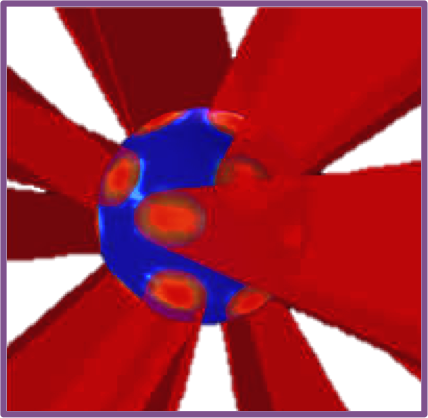
\includegraphics[scale=.95]{graphics/laserFusion.png}
	\caption[Inertial Confinement Fusion]{ \\ Inertial Confinement Fusion \\ \captiontitlefinal{\textmd{is sometimes referred to as laser-driven fusion because it involves shooting a millimeter-sized target with an array of lasers. This image captures how the areal projections of the lasers impact the spherical symmetry of the problem \citep{aNewShock}. } } }
	\label{fig:laser}
\end{SCfigure}

After ignition, the fuel source continues to burn until a dismantling shockwave - originating at the center - has a chance to propagate outwards.  Once this shockwave reaches the target`s shell, it ruptures the surrounding plasma envelope and causes the target to explode.  The optimization problem at hand, then, is to maximize the number of fusion reactions that occur in the nanoseconds-length time window between the target`s ignition and subsequent explosion.

In order to develop a working inertial fusion reactor, though, many implementation decisions and technologies still need to be made.  Several research facilities exist to investigate such issues, most notably the one at the National Ignition Facility in Livermore, California (Fig.\,\ref{fig:nif}).  At these facilities, one issue that gets a considerable amount of research attention is the type of ignition.  

\begin{SCfigure}[][h!]	
	\centering
	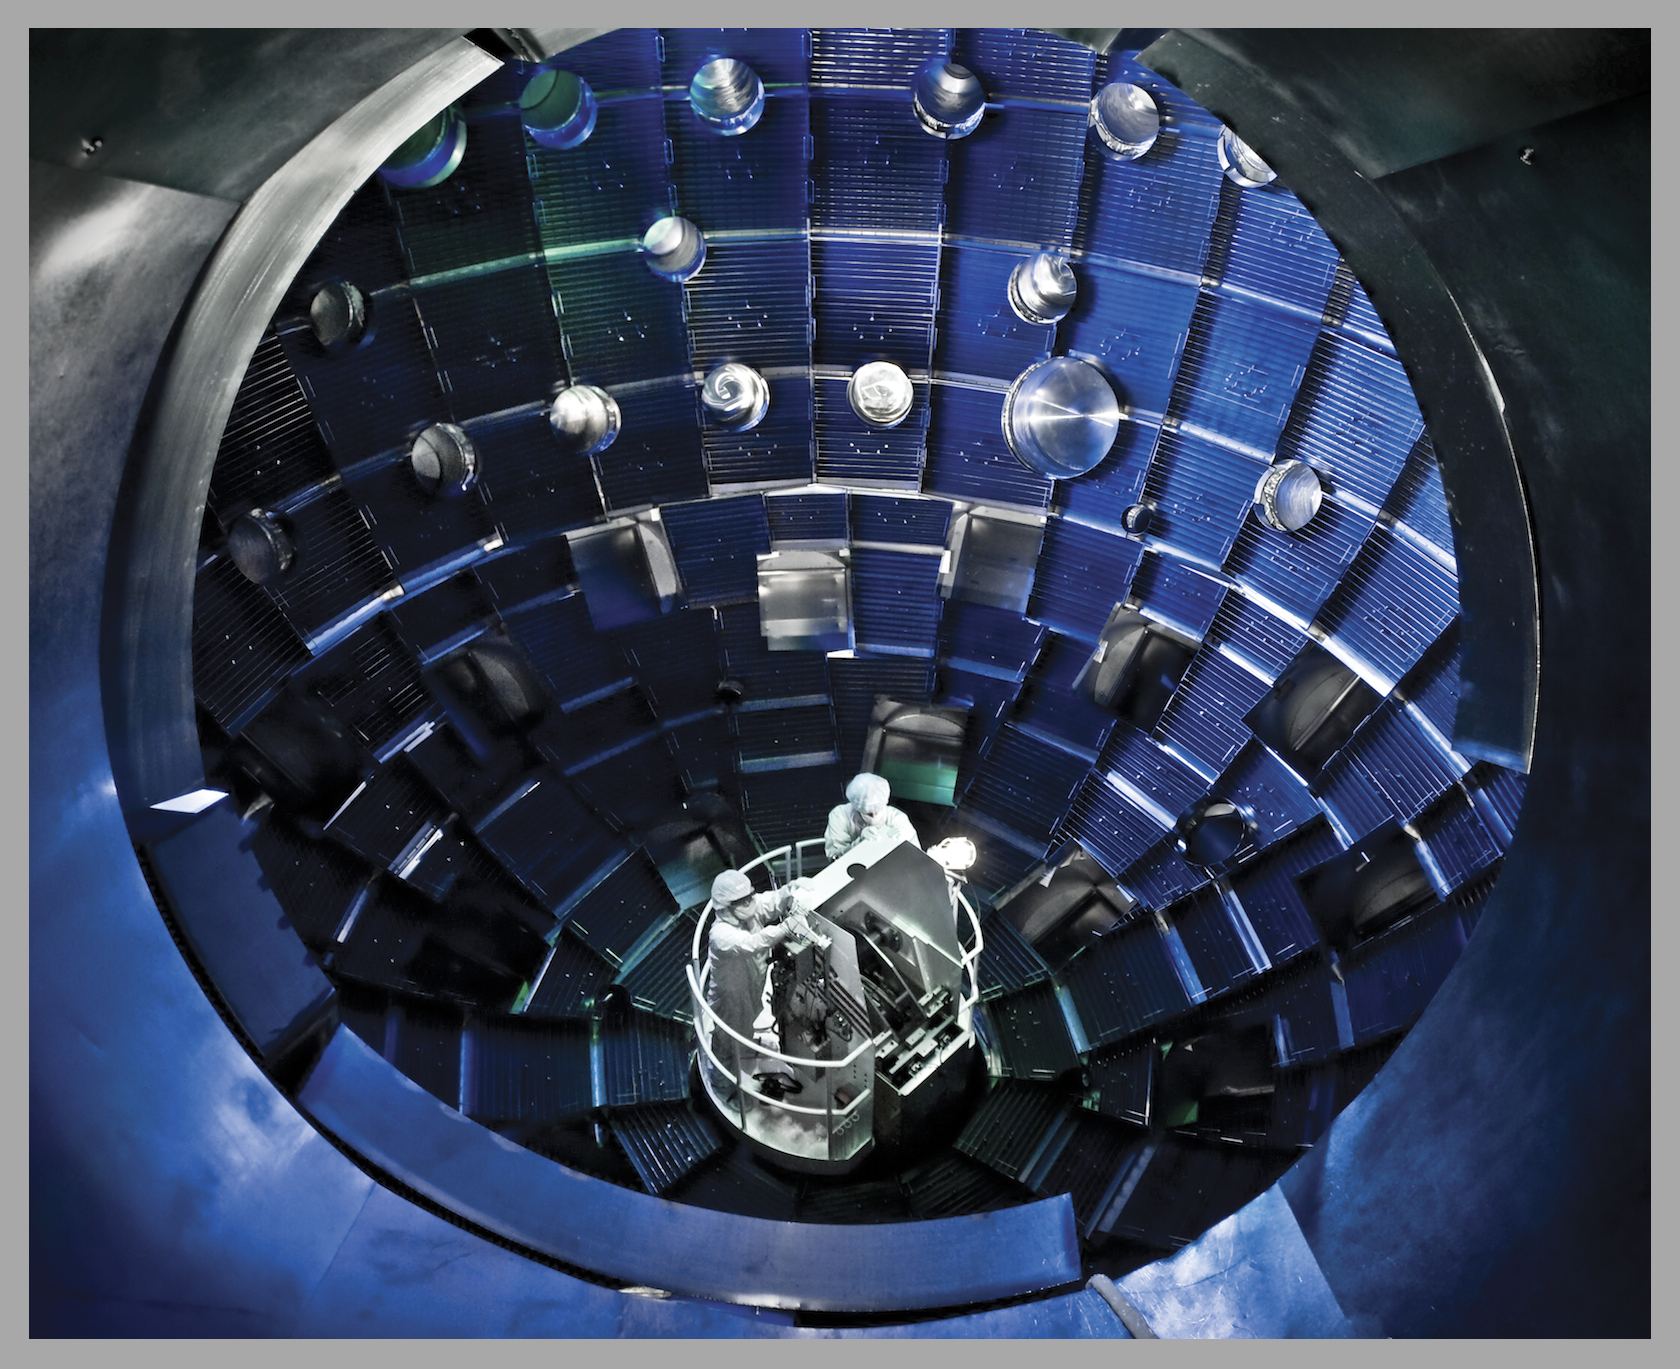
\includegraphics[scale=.4]{graphics/nif.jpg} 
	\caption[The National Ignition Facility]{ \\ The National Ignition Facility \\ \captiontitlefinal{\textmd{houses the world's largest laser array.  Inside the holes of the spherical chamber are nearly two-hundred lasers.  At roughly ten meters, the chamber itself is four orders of magnitude larger than the plastic targets it ignites. } } }
	\label{fig:nif}
\end{SCfigure}

Currently, the two most common types of ignition are direct drive and indirect drive.  In direct drive ignition, the laser array focuses directly on a target; while in indirect drive ignition, the laser array focuses on a gold shell surrounding the target that then deposits X-rays onto the target.  Although these two types of ignition are the most common, others exist: one prospective type being shock ignition \citep{summaryPaper}. 

\section{Achieving Ignition with Aligned Shock Fronts}

Shock ignition gets its name from how it achieves ignition: by timing shockwaves so that they add constructively at the center of a fuel target. The reason these shockwaves are able to reach a specific location simultaneously is because of their different speeds.  

In shock ignition, shockwaves are produced asynchronously by fluctuations in laser power.  Therefore, to have each shockwave coalesce at a certain radius later on, faster and faster wave speeds are needed for each successive shock.  Because these wave speeds are positively correlated to laser power, shock convergence can be achieved with a laser profile of individual pulses that increase in power. This then transforms the problem of aligning shockwaves into one of tuning a laser array's power versus time profile \citep{terryThesis}.  

This problem of constructing a laser array's power vs.\ time profile is the fundamental difference between shock ignition and other leading ignition schemes.  In conventional schemes for ignition, laser array profiles are designed to couple the compression stage and the ignition stage of the target, while in shock ignition, the profiles are designed to decouple them \citep{perkinsPaper}. 

As shown in Fig.\,\ref{fig:laserProfile}, this decoupling is accomplished by dividing the main laser pulse, which accounts for most of the energy consumption, into two separate pulses: a compression pulse and an igniter pulse.  The compression pulse, which is a relatively long, weak pulse, is designed to heat and to compress the target.  While, the igniter pulse, which is a relatively quick, high intensity burst, is designed to actually cause the target to ignite.  This decoupling of the two pulses leads to shock ignition having several unique characteristics when compared to other forms of ignition.  

\sidecaptionvpos{figure}{c}

\begin{SCfigure}[][h!]	
	\centering
	\caption[Laser Power versus Time Profiles]{ \\ Laser Power vs. Time \\ Profiles for Shock Ignition \\ and Direct Drive Ignition. \\ \captiontitlefinal{\textmd{Shock ignition differs from Direct Drive ignition in the way its laser profile is constructed.  Shock ignition separates what would be the main pulse into two pulses, which consequently decouples the target's compression stage and its ignition stage \citep{perkinsPaper}. } } }
	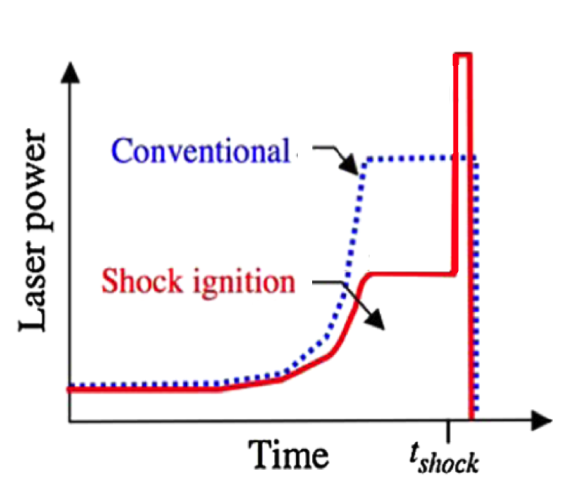
\includegraphics[scale=1]{graphics/laserProfile.png} 
	\label{fig:laserProfile}
\end{SCfigure}

\pagebreak

The major advantage shock ignition has over other competing ignition schemes is that its targets prospectively produce higher net gains, see Fig.\,\ref{fig:gainCurve}.  Here, a gain is defined as the ratio of fusion energy produced to the driver energy incident on the target, where a higher gain would correlate to a higher return of energy \citep{mosesBook}.  

\begin{SCfigure}[][h!]	
	\centering
	\caption[Gain Curve for Shock Ignition]{ \\ Gain as a function of \\ Laser Energy for Shock Ignition.   \\ \captiontitlefinal{\textmd{Early 1-D simulations show that the gains from shock ignition targets not only exceed the NIF baseline requirements, but also surpass those of candidate targets for both direct drive ignition (DD) and polar direct drive ignition (PDD) by nearly an order of magnitude \citep{perkinsPaper}. } } }
	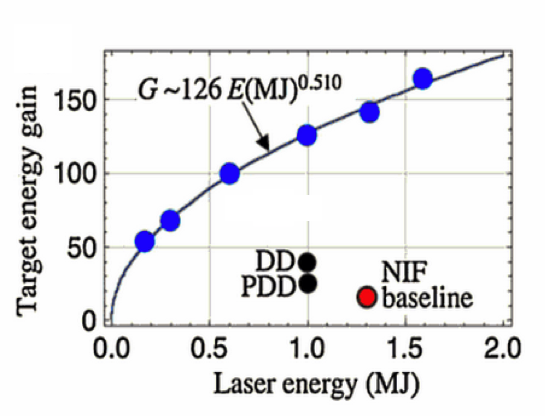
\includegraphics[scale=0.95]{graphics/gainCurve.png} 
	\label{fig:gainCurve}
\end{SCfigure}

\sidecaptionvpos{figure}{b}

Shock ignition is capable of achieving these gains because its targets have longer burn times, a consequence of the relatively low implosion velocities and thick instability-resilient shells inherent to the process \citep{perkinsPaper}.  A corollary of these high gains is that a feasible shock ignition reactor could produce the same amount of energy as any other potential inertial fusion reactor with a much weaker, and thus a much cheaper, laser \citep{summaryPaper}.  

In order for shock ignition to actually achieve these gains, though, its laser array's power versus time profile has to be constructed properly.  This construction process entails combining several laser pulses together in a very specific configuration.  Here a laser pulse is a section of the power versus time profile that has some definite shape, such as a horizontal line or a Gaussian curve.  

In addition to being constructed properly, a laser profile needs to be constructed efficiently.  There are several reasons for this.  First, because time at inertial fusion research facilities is expensive, many simulations are needed to justify every set of experiments.  Second, because there are so many research branches, e.g. target design and polar drive, the number of simulations needs to be minimized.
